\documentclass{styles/sig-alternate}

\usepackage{times}
\usepackage{epsfig}
\usepackage{subfigure}
\usepackage{balance}
\usepackage{color}
\usepackage{graphicx}
\usepackage{fancyvrb}
\usepackage{mdwlist}

\newcommand{\ignore}[1]{}
\newcommand{\boldheading}[1]{{\vspace{0.1in}\noindent \bf #1} \hspace{0.06in}}
\newcommand{\somecode}[1]{{\vspace{0.1in}\noindent \bf \tt #1} \hspace{0.02in}}

\renewcommand\topfraction{.95}
\renewcommand\textfraction{.05}
\renewcommand\floatpagefraction{.95}
\renewcommand\bottomfraction{.95}

\hyphenation{cach-ing}
\pagenumbering{arabic}

\makeatletter
\let\@copyrightspace\relax
\makeatother

\begin{document}
\title{Iterative Stencil Language Compiler}
\author{
\alignauthor Greg Faust and Sal Valente\\
\affaddr{CS 6620: Compilers\\
University of Virginia}
}
\maketitle

\begin{abstract}

Over the last several years it has become clear that performance gains through hardware and 
software exploitation of instruction level parallelism has reached a plateau.  
Instead, attention has shifted toward performance gains from multi-core hardware 
architectures and software tools to exploit thread and/or task level parallelism.  
Research into automatic techniques to recapture such parallelism from programs written 
in standard sequential languages such as C or Java is ongoing.  However, it is also useful 
to consider the benefits of new language constructs that make it easier for programmers 
to express such parallelism without the need to attend to all the complexity of 
writing parallel algorithms.  Here we present a new language is which users can easily 
express computations that involve iterative stencil calculations.  
Such computations form an important subset of parallel algorithms and are 
widely used in scientific, engineering and other important application areas.


Specifically, we present the Iterative Stencil Language (ISL).  
Using ISL, a programmer need only express the central kernel of their 
computation, not an entire parallel program for it.  We have also built a 
translator for ISL capable in principal of translating the ISL program into code for 
different parallel programming models.  
We provide an initial translation into the C++ extensions of the CUDA programming 
model for nVIDIA GPUs.  Further, the CUDA code is automatically dynamically optimized 
for the current execution environment.  The optimizer is an extension of an analytical 
model for CUDA stencil applications originally developed by Meng and Skadron \cite{meng}, 
that is now capable of using dynamic information about the application and the specific 
GPU the application is running on.  
Finally, we validate the compiler and the optimizer through performance evaluation of the resultant code.

\end{abstract}

\section{Introduction}

{\em Iterative stencil loops} (ISLs) \cite{li} are a class of loops
that are commonly used in fields including numerical simulations and
signal processing.  ISLs usually operate on matrices with one, two, or
three dimensions.  An ISL calculation takes an input matrix $m_{in}$
and produces an output matrix $m_{out}$.  The calculation has the
following properties:

\begin{enumerate*}
\item $m_{in}$ and $m_{out}$ have the same number of dimensions and
  the same size.
\item Each value in $m_{out}$ is calculated independently of each
  other value.
\item There is a single function which is used to calculate each value
  in $m_{out}$ regardless of the coordinates of the value.
\end{enumerate*}

For example, say that $m_{in}$ is a two-dimensional matrix.  Say that
the stencil calculation is defined as: ``$m_{out}[x, y] =$ the average
of the north, south, east, and west neighbors of $m_{in}[x, y]$.''
Then this function will be calculated for every cell in $m_{out}$.

The {\em stencil} is the set of cells in the input matrix, relative to
the coordinates of the cell which is being calculated, that is used in
the stencil calculation.  In the above example, the stencil is a set
of four cells: The north, south, east, and west neighbors.

The process of calculating a complete output matrix is called an {\em
  iteration} or a {\em time step}.  At the end of an iteration, we can
take the output matrix $m_{out}$ and use it as the input matrix to the
next iteration.  This loop can continue for as long as necessary.
Some iterative stencil loops are defined to run for a predetermined
number of time steps.  Other stencil loops are defined to run until
the values converge.

Stencil calculations are data parallel.  Since each value is
calculated independently of each other value, the values can be
calculated in any order or at the same time.  If the matrix has $n$
cells and the computer has $n/k$ processing elements (PEs) available,
then each processor only needs to calculate a block of size $k$.  This
partitioning of the matrices among multiple processors is called
{\em tiling}, and the block calculated by a processor is called a
tile.

When a PE calculates a given tile for many iterations, that PE can
take advantage of both spatial locality and temporal locality.
\begin{itemize*}
\item {\bf Spatial locality.} As a general rule, stencil calculations
  read each input value multiple times.  For example, say that the
  stencil is defined as the cell's left and right neighbors.  When a
  PE calculates the value of a cell at $x=0$, it reads that value of
  that cell's right neighbor at $x=1$.  Then, when it calculates the
  value of a cell at $x=2$, it reads that cell's left neighbor, which
  is the value at $x=1$ again.  Thus, a PE can optimize this
  computation by keeping input values in a local cache.
\item {\bf Temporal locality.} If a PE generates an output value
  during iteration $x$, then that PE can use that value as an input
  value during iteration $x+1$.
\end{itemize*}

Unfortunately, stencils along the boundary of a tile cannot find all
of their input values in the local processor cache.  These stencils
must obtain values that were computed on other PEs.  The regions of
data that must be exchanged are called {\em halo} regions.  As a
result of this exchange, ISL algorithms may spend considerable time
stalled due to communication and synchronization delays.

\begin{figure}
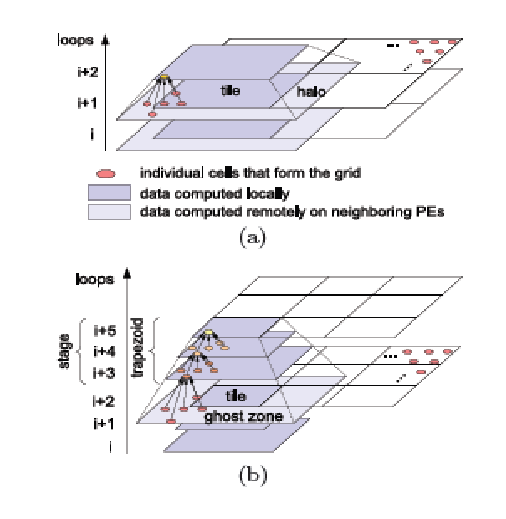
\includegraphics[clip,trim=1in 1.2in 1in 1.2in,width=3.3in]{StencilDiagram}
\caption{(a) Iterative stencil loops and halo regions.  (b) Ghost zones help
reduce need for global synchronizations.  Note: this figure originally appeared in \cite{meng}
and is reprinted here with the Authors' permission.}
\label{fig:Stencil}
\end{figure}

A solution to this problem is to include a {\em ghost zone} in each
tile.  A ghost zone is a perimeter around the tile which overlaps
neighboring tiles.  The overlap allows each PE to generate its halo
regions locally for one or more iterations.  Specifically: Say that a
processor is responsible for calculating a tile with $n$ cells.  As
input, the processor is given a larger tile with values in those $n$
cells and also in $x$ halo regions around those cells.  The processor
can execute $x$ iterations without communicating with any other
processor, and it will end up with valid values in the $n$ cells in
the output tile.  See Figure ~\ref{fig:Stencil}.

In the paper ``Performance Modeling and Automatic Ghost Zone
Optimization for Iterative Stencil Loops on GPUs,'' \cite{meng}
Jiayuan Meng and Kevin Skadron wrote:

\begin{quote}
Ghost zones pose a trade-off between the cost of redundant computation
and the reduction in communication and and synchronization between
PEs.  This tradeoff remains poorly understood.  Despite the ghost
zone's potential benefit, an improper selection of the ghost zone size
may negatively impact overall performance.
\end{quote}

Meng and Skadron examined the problem of writing efficient ISL code in
the CUDA language to run on an nVIDIA GPU.  They defined a mathmatical
model for calculating the optimal ghost zone size.  Unfortunately, the
model is hard to use.  It has roughly a dozen parameters, and some of
them are difficult to calculate both at compile time and at runtime.

To summarize, writing efficient ISL code is hard for these reasons:
\begin{itemize*}
\item The code must use tiling to take advantage of spatial locality.
  Tiling can be hard and calculating the optimal tile size can be
  hard.
\item The code must use ghost zones to avoid communication delays.
  Writing ghost zones can be hard and calculating the optimal ghost
  zone size can be very hard.
\item The code must be optimized for a particular environment.  The
  optimal ghost zone size on an old GPU might be different from the
  optimal size on a new GPU which might be different from the optimal
  size on a multicore CPU.
\end{itemize*}

The goal of our research is to define and create tools which make it
easy to write ISL code.  The programmer of a stencil calculation
should not need to write code to calculate the optimal ghost zone
size.  In fact, he should not need to write any code that is in any
way related to tiling or ghost zones.  Nor should he need to write
code to optimize spatial or temporal locality for one or more
environments or architectures.  It should be possible to implement an
efficient ISL simply by describing the stencil and the stencil
calculation.

We have achieved these goals.  Our contributions are as follows:
\begin{itemize*}
\item We have defined a {\em stencil language}.  This is a formal
  high-level language in which a programmer can describe an ISL
  computation.  By design, a description written in the language must
  include all of the information necessary to calculate the correct
  results, and none of the information that would tie its performance
  to a particular architecture.
\item We have created a stencil language compiler.  The front-end of
  the compiler parses the stencil file.  The back-end outputs
  efficient CUDA code.
\item The CUDA code calculates the optimal ghost zone size.  It's
  built using the model defined by Meng and Skadron.
\item We have refined the model to collect as much information as
  possible dynamically at runtime.  This allows the generated code to
  calculate good values on a variety of GPU cards, and it should allow
  the code to continue to work well with future hardware.
\item We have designed our compiler so that it can be extended with
  multiple back-ends.  Based on a single source file, it could output
  efficient code for CUDA or OpenMP or pthreads or other environments.
\end{itemize*}

The remainder of this paper is organized as follows.  Section 2
discusses related work.  Sections 3 through 5 describe our
contributions.  Section 3 is the complete definition of our stencil
language.  Section 4 presents the design and implementation of our
stencil language compiler.  Section 5 discusses the CUDA code which is
generated by the compiler, including the code which calculates the
optimal ghost zone size.  Section 6 discusses the performance of the
generated code.  It contains our experimental setup and results.
Section 7 concludes.

\section{Related Work}

As stated in the introduction, our work is directly related to that of
Jiayuan Meng and Kevin Skadron \cite{meng}.  They defined the model
which we have implemented.

Zhiyuan Li and Yonghong Song may have been the first to use the term
{\em iterative stencil loops} \cite{li}.  They developed a compiler
framework for these loops that used tiling to improve temporal data
locality.  Their work was intended to be run on a uniprocessor, so
they did not face any communication costs and they did not consider
ghost zones.

We are not the first to create a stencil compiler.  A group at Harvard
created a stencil compiler for the Connection Machine CM-2 massively
parallel architecture \cite{cm2}.  The stencil expression was
expressed for their compiler in a ``microcode'' which was specific to
the CM-2 architecture.  (TODO: This paper is a hard to understand.  We
should say how their goals and language differ from our goals and
language.)

Shoaib Kamil et al. studied the effects of tile size and time skewing
to increase memory locality on the Itanium2, Opteron, Power5, and Cell
\cite{kamil}.  They concluded that controlling tile size and data
locality reuse across time slices is critical to performance.  In
addition, they concluded that when hand optimizing, better performance
is achievable on the Cell because of the users’ explicit control of
the memory hierarchy.

Paulius Micikevicius from nVIDIA explored the hand coding of stencil
applications on CUDA, and in particular the desired sizes of ghost
zones around the array tiles \cite{Micikevicius}.  He also
investigated using asynchronous data transfers and computations for
array sizes too large to fit in GPU global memory.  In a somewhat
related area, Vasily Volkov investigated in great detail hand
optimizations of CUDA programs involving parallel operations on large
arrays \cite{volkov}.  For our project, we have done manual
optimizations similar to those presented by Micikevicius and Volkov so
that the user of our compiler does not need to be aware of them.

TODO - I haven't looked much at Micikevicius's and Volkov's papers.
Is the above paragraph accurate?

Several attempts have been made to build simplifying layers on top of
the CUDA language.  At Purdue, they built a source-to-source
translator for OpenMP to CUDA \cite{openmp}.  OpenMP is a
standards-based set of language extensions targeted at expressing
parallel computations on shared memory architectures.  OpenMP can
express a significantly wider range of parallel computations then that
which can be expressed by our stencil language, but an OpenMP
translator cannot optimize specific computations in the way that our
compiler does.

CUDA-lite is a general purpose source-to-source translator for
automatically optimizing CUDA programs \cite{cudalite}. The user
expresses his program in CUDA syntax, but using only the most general
and easy to use level of the CUDA memory hierarchy, namely the global
memory space.  This is by far the largest and most accessible of the
memory spaces, so it is easier to write CUDA programs that solely use
this memory space is easier than to write programs optimized for the
smaller, faster memory spaces.  With CUDA-lite, the user includes some
additional pragmas in his code that gives hints to CUDA-lite about the
size, shape, and access of the global memory arrays.  Then CUDA-lite
generates a CUDA program that takes advantage of the special memory
spaces, generally resulting in a factor of 3X speedup.

\section{Stencil Language}

\begin{figure}
\begin{small}
\begin{verbatim}
NumDimensions 2
StencilSize (1, 1)
DataType float
FunctionName runHotspot

ScalarVariables (
  float Rx, float Ry, float Rz
}

CellValue {
  float pvalue, value, term1, term2, term3, sum;
  pvalue = read(y * input_size.x + x);
  value = get(0, 0);
  term1 = (get(0, 1) + get(0, -1) - value) / Ry;
  term2 = (get(1, 0) + get(-1, 0) - value) / Rx;
  term3 = (80.0 - value) / Rz;
  sum = pvalue + term1 + term2 + term3;
  return(value + sum);
}

EdgeValue {
  return value;
}
\end{verbatim}
\end{small}
\caption{The hotspot.sl stencil language file.  This example
  shows a description of a two-dimensional stencil calculation where
  the value of each cell is based on the values of that cell's
  immediate neighbors.  The read-only data is interpreted as a
  two-dimensional matrix which indicates that some areas of the chip
  inherently run hotter then other areas.}
\label{fig:hotspot} 
\end{figure}

\subsection{Syntax}

A stencil language file is a plain text line-oriented file that
contains a set of key-value pairs.  The key and value are separated by
whitespace.  A key is an alphanumeric string.  A value can be:
\begin{itemize*}
\item an integer
\item a string of alphanumeric and underscore characters
\item an array of scalars, inside parentheses, separated by commas
\item a block of C code inside of curly braces
\end{itemize*}
Comments start with {\tt //} and go to the end of the line.

\subsection{Content}

\begin{itemize}
\item {\bf NumDimensions} -- A stencil may have 1, 2, or 3 dimensions.
\item {\bf StencilSize} -- The size of the stencil in each dimension.
  If the stencil size is 1 in the $x$ dimension, then the value of the
  cell at $(x, y)$ may be based on the previous iteration's values of
  the cells in the $x-1$ and $x+1$ coordinates.
\item {\bf DataType} -- The data may be 32 bit or 64 bit integers or
  floating point numbers.  The values are {\tt int}, {\tt int64}, {\tt
    float}, and {\tt double}.  Values may be signed or unsigned.
\item {\bf FunctionName} -- The name of the function that will be exported
  from the generated .cu file.  The first argument to the function,
  {\tt data}, will be a matrix of the specified data type with the
  specified number of dimensions.  As input to the function, {\tt
    data} must contain the initial state of the problem.  It must
  contain valid data in each of the $x \times y \times z$ cells.  As
  output from the function, it will contain the final data.  The next
  $n$ arguments to the function are the input sizes in each dimension.
  The next argument is the number of iterations to run.
\item {\bf ScalarVariables} -- A list of numeric variables that will
  be arguments to the exported function after {\tt data, x, y, z,
    iterations}.  The caller will pass these arguments to the
  function, and then the stencil calculator will be able to use these
  variables (read-only) in its calculations.
\item {\bf CellValue} -- A block of C code that will be run for every
  cell in the data set in every iteration.  The code has access to the
  following variables and functions:
\begin{itemize}
\item {\tt x, y, z} -- The coordinates of the current cell in each
  dimension.
\item {\tt iteration} -- The iteration number.  Since iteration 0 is
  given as input, this code will first be called with {\tt iteration}
  = 1.
\item {\tt input\_size} -- a structure with {\tt x}, {\tt y}, and {\tt
  z} fields, containing the total size of the input
\item All variables listed in the {\bf ScalarVariables} field.
\item {\tt get(...)} -- a function that efficiently returns values
  from the stencil from the previous iteration.  The parameters are
  relative to the current cell.  For example, in a two-dimensional
  stencil, the west and east neighbors can be retrieved with {\tt
    get(-1, 0)} and {\tt get(1, 0)}.
\end{itemize}
The block of code returns the new cell value.
\item {\bf EdgeValue} -- A block of C code that returns the cell value
  of cells that are outside the bounds of the input.  This code has
  access to the same variables as the {\bf CellValue} code.  Note that
  at least one of {\tt x}, {\tt y}, or {\tt z} will be out of bounds
  -- it will be either less than zero or greater than or equal to the
  size of that dimension.  This code may not use the {\tt get()}
  function.  Instead, it can access the {\tt value} variable, which
  will contain the value of the nearest cell in bounds from the
  previous iteration.
\end{itemize}

\subsection{Unnamed Data}

The generated .cu file will export two functions.  One of the
functions will have the given function name.  The other function will
have the function name appended with {\tt SetData}.  For example, if
the stencil language file says:
\begin{verbatim}
FunctionName runStencil
\end{verbatim}
then the generated .cu file will export these two functions:
\begin{itemize*}
\item {\tt runStencil()}
\item {\tt runStencilSetData()}
\end{itemize*}

\noindent The SetData function takes two arguments:
\begin{enumerate*}
\item An array of elements of the specified data type
\item The number of elements in the array
\end{enumerate*}
If a program calls the {\tt runStencilSetData()} function with an
array, and then the program calls {\tt runStencil()}, then the stencil
calculator will have read-only access to this data in the array.  The
{\bf CellValue} code can access the $i$th read-only data element by
calling {\tt read(i)}.

\subsection{Example Source File}

Figure~\ref{fig:hotspot} shows a stencil language description of the
``hotspot'' calculation.  This code calculates the temperature
patterns in a two-dimensional microchip where the current state is a
function of the previous state, the edge values, and a two-dimensional
read-only ``power usage'' matrix.

\section{Stencil Language Compiler}

We implemented the stencil language compiler in less than 600 lines of
Java code.  This is what it does:
\begin{enumerate*}
\item Convert a stencil language file into a token stream
\item Parse the token stream into a symbol table
\item Read a plain text template file
\item Output a new file which contains the template integrated with
  the stencil description
\end{enumerate*}

Step 1 is implemented by {\tt Tokenizer.getToken()}.  A token is
either a string of alphanumeric characters or any symbol token that's
in the language such as parentheses, commas, etc.  Also, the tokenizer
can recoginize comments and blocks of C code.

Step 2 is implemented by {\tt Stencil.parse()}.  It runs a loop that
reads a key and then parses a value, which may be an integer, a
string, a list, or a block.  The parser verifies that the key is
defined by the language and that the value has the right type for that
key, and then it adds the key value pair to a symbol table.

Step 3 is implemented by the creator method of the {\tt Template}
class.  It stores the template text in the Template instance.

Step 4 is implemented by {\tt Template.applySymbolTable()}.  It looks
for instances of {\tt @name@} in the text.  For each instance that it
finds, it looks up {\tt name} in the symbol table, and it replaces the
variable with the value.

This design is flexible.  It can easily support multiple architectures
and optimizations.  We have written templates for CUDA code for 1-D,
2-D, and 3-D stencil calculations.  These templates are written such
that the {\bf CellValue} code can be dropped-in unmodified.  The code
in these templates is optimized for shared memory usage, and it
calculates the optimal ghost zone size.  We have also written a
template which does not use shared memory, so that we could compare
its performance to that of the optimized templates.

We are confident that an OpenMP template could be written without
requiring any changes to either the stencil language or the compiler.

\section{CUDA Templates}

\subsection{ISL Calculations}

TODO

\subsection{Ghost Zone Size Calculation}

TODO

\section{Experimental Results}

Our primary goals for this research were to define a stencil language, provide a compiler for it, 
and to statically and dynamcilaly optimize the generated programs in terms of the use of GPU shared memory, 
tile size and pyramid height within the target set of GPU architectures for which the peformance model was 
originally developed.  It was not our goal to improve the performance of the optimizer to a broader set of 
nVIDIA GPU cards.  Therefore, we restricted our testing to the original target environment for the optimizer.
Out testing environment is a ???? processor running Linux 2.6.24, with an installed GTX-280 nVIDIA GPU running 
version 2.2 graphics driver.  The GTX-280 has 30 PEs each of which has 8 SIMD cores and can handle up to 8 
concurrent running blocks, with maximum block size of 512 threads.  It has a clock speed of 1.3GhZ, and 1GB of
global memory.  All code was compiled with the nVIDIA provides NVCC compiler driver which in turn 
calls GNU tools for compiling C++ code and linking.  The installed GNU tools were version 4.2.4, and all code was
compiled with -O3.

We use the same four stencil applications as Meng did in his orginal study.  They are described below.
All of the graphs of runtimes vs pyramid height have the same basic curve.  Very low pyramid heights are not
large enough to take advantage of all available spatial and temporal locality, and perform worse than larger
pyramid heights.  However, beyond some optimal pyramid height, the runtimes again increase due to the overhead
of all the ghost zone calculations that are thrown away at the global synchromnization point.  Another way to
see this trade-off is that with increased pyramid height, the number of threads per tile that calculate final cell 
values drops off at twice the size of the stencil per dimension per pyramic height (see Figure ~\ref{fig:trapezoid}).  Therefore, 
for very large pyramid heights the effective tile size gets smaller, and the total number of tiles, and therefore
also the total number of threads increases.  Eventually, in the limiting case, the pyramid height is so high that 
{\em no} useful cell values are calculated!  Near this extreme, run times increase exponentially.


\begin{enumerate*}
\item The first test case is a 1D stencil application called ``Pathfinder'' that performs a dynamic programming calculation 
of the lowest cost of any vertical path through a two dimensional grid of data.  
The 2D input data set is read-only data during the CellValue computation.  
Each iteration of the main loop calculates the min costs down another row in the 2D grid.
The tiles are horizontal slices across the columns of the 2D grid.  As this is a 1D application,
the x dimension of the tile size can be up to 512 cells (threads).  Therefore, theoretically possible
pyramid heights vary from 1 to 255.  Figure ~\ref{fig:pathfinder} shows the runtimes vs pyramid heights for pathfinder for
row width of 100,000 and 400,000.  As with all the applications, these large sizes are chosen to ensure
that the GPU is saturated with threads.  Meng originally also ran this at 700,000 and 1,000,000 as did we.
However, the latter two data sets have been left out of the chart, as they have the same shape, and are enough
larger in magnitude that their inclusion would compress the detail that is most important to see.  For the same
reason, pyramid heights above 235 are not shown as they raise so dramatically that they would again compress
the interesting part of the curve.  


Notice that the valley for the main portion of this curve is very shallow.  Therefore, it 
is hard for the model to accurately predict the exact best pyramid height.  And in fact, our model does not.  For the 100,000 column data set,
the measured best pyramid height is 16, our model predicts 18 with a resultant loss of performance of 2.79\%.  For the 400,000 column data set,
the measured best height is 17, our predicted height is 21, with a resultant loss of performance of 2.74\%.  For the 700,000 column data set,
the measured best height is 12, while our predicted height is 20, but still this only results in a performance loss of 1.0\%.  Finally, for the
million column data set, the measured best height is 14, while we predict 19, with a resultant loss of 0.99\% in performance.  From these results, one
can see that the shape of the interesting part of the curve is so flat that precise pyramid height prediction is not necessary to result in very positive results.
For comparison, the naive use of a pyramid height of 1 for the 1,000,000 column data set would result in a performance loss of 43\%.
\item The second test case is a 2D stencil application called ``HotSpot''.  The ISL for this application is show in Figure 2.  
The application models heat 
\end{enumerate*}


\begin{figure}
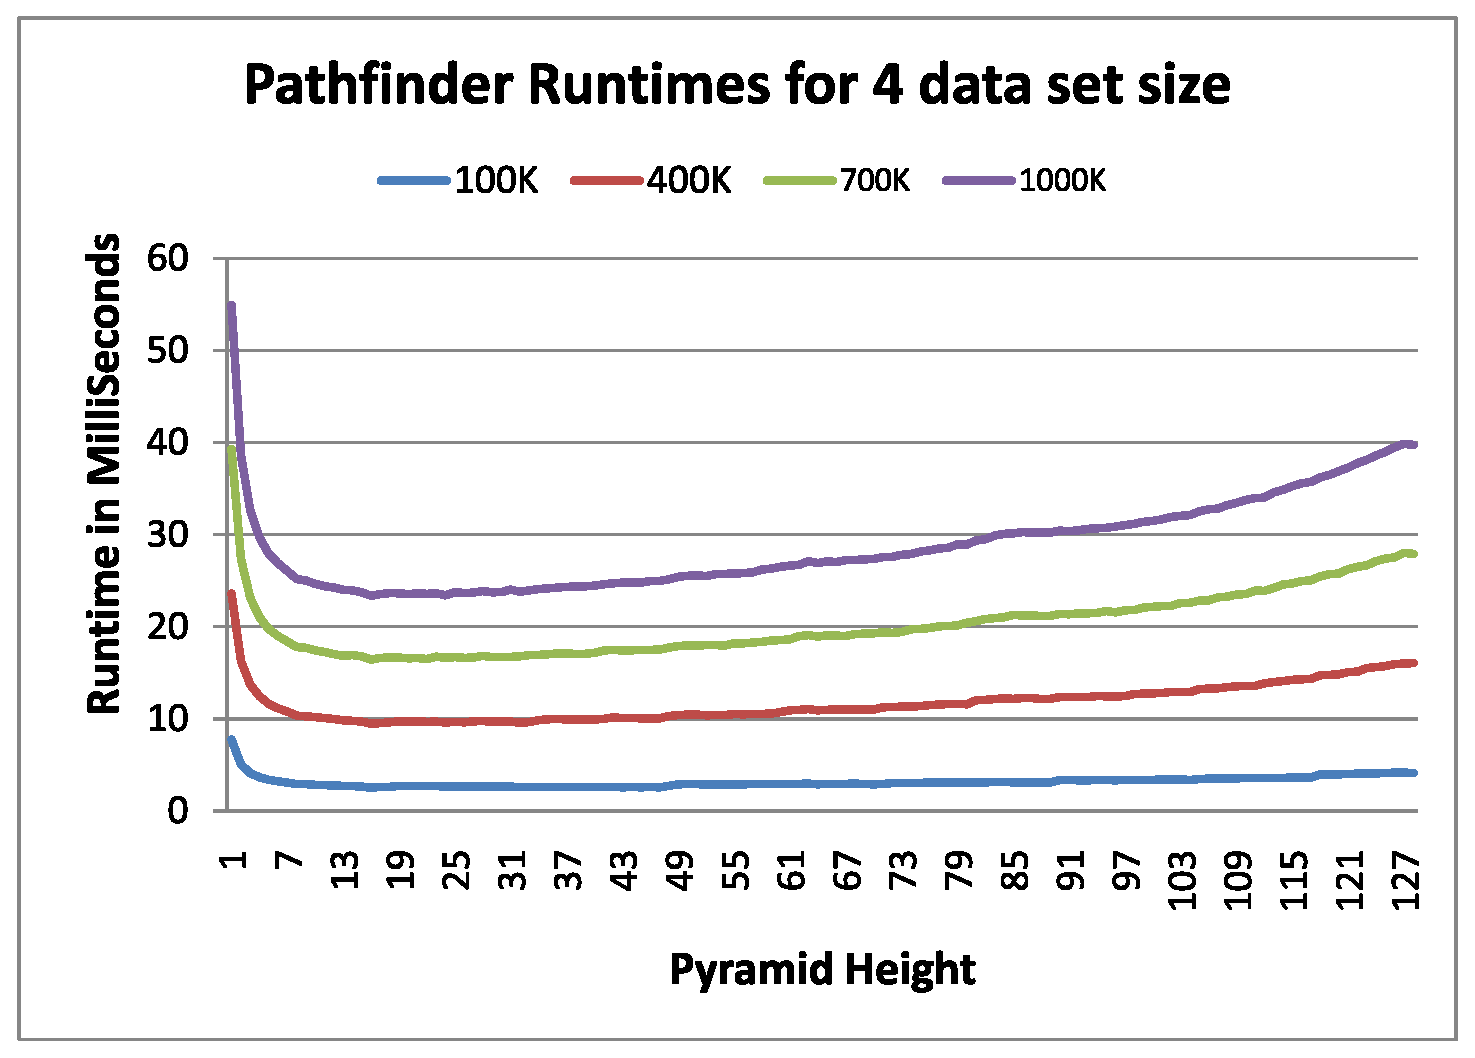
\includegraphics[clip,trim=1in 1in 1in 1in,width=3.3in]{PathfinderTimingData}
\caption{This chart shows the actual measured runtimes for the Pathfinder 1D stencil appliction vs pyramid height.
As can be seen, the lowest portion of the curves are very flat.  Therefore, even though our analytical model did not 
accurately pick the best pyramid height for any data set size, the resultant performance was between 0.99\% and 2.79\% of optimal.}
\label{fig:pathfinder}
\end{figure}

TODO

\section{Conclusion}

TODO

\balance
\bibliographystyle{abbr}
\bibliography{report}
\end{document}
